\documentclass[a4paper,12pt]{article}

\usepackage[utf8x]{inputenc}
\usepackage[T2A]{fontenc}
\usepackage[english, russian]{babel}

% Опционно, требует  apt-get install scalable-cyrfonts.*
% и удаления одной строчки в cyrtimes.sty
% Сточку не удалять!
% \usepackage{cyrtimes}

% Картнки и tikz
\usepackage{graphicx}
\usepackage{tikz}
\usetikzlibrary{snakes,arrows,shapes}


% Некоторая русификация.
\usepackage{misccorr}
\usepackage{indentfirst}
\renewcommand{\labelitemi}{\normalfont\bfseries{--}}

% Увы, поля придётся уменьшить из-за листингов.
\topmargin -1cm
\oddsidemargin -0.5cm
\evensidemargin -0.5cm
\textwidth 17cm
\textheight 24cm

\sloppy

% Оглавление в PDF
\usepackage[
bookmarks=true,
colorlinks=true, linkcolor=black, anchorcolor=black, citecolor=black, menucolor=black,filecolor=black, urlcolor=black,
unicode=true
]{hyperref}

% Для исходного кода в тексте
\newcommand{\Code}[1]{\texttt{#1}}

\usepackage{verbatim}
\usepackage{fancyvrb}
\fvset{frame=leftline, fontsize=\small, framerule=0.4mm, rulecolor=\color{darkgray}, commandchars=\\\{\}}
\renewcommand{\theFancyVerbLine}{\small\arabic{FancyVerbLine}}


\title{Отчёт по лабораторной работе \\ <<IP-маршрутизация>>}
\author{Ван Пэнфэй}

\begin{document}

\maketitle

\tableofcontents

% Текст отчёта должен быть читаемым!!! Написанное здесь является рыбой.

\section{Топология сети}

Топология сети и использыемые IP-адреса показаны на рис.~\ref{fig:network}.

\begin{figure}
\centering
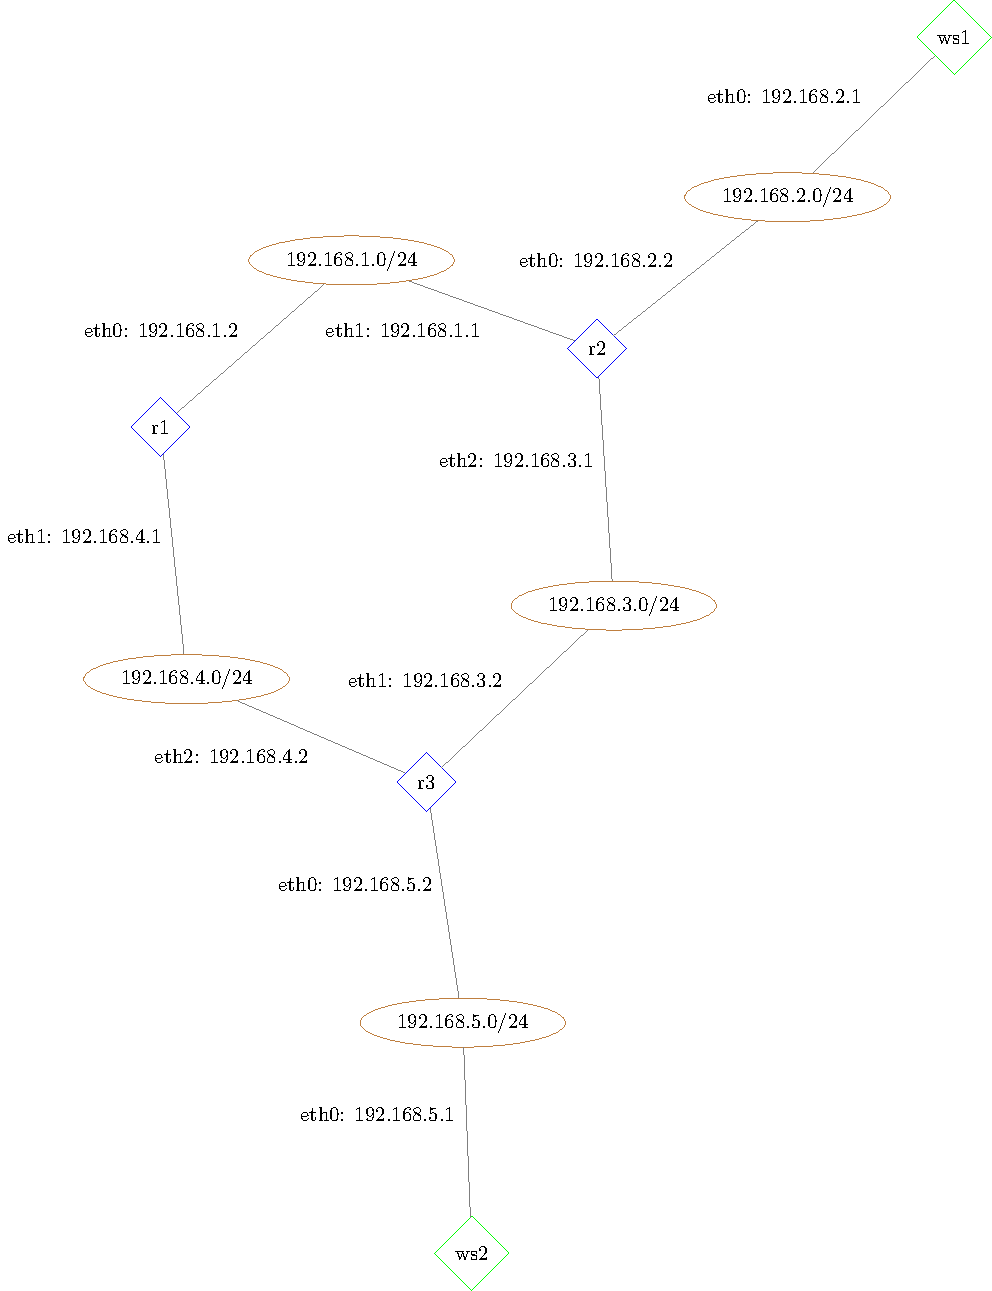
\includegraphics[width=\textwidth]{includes/network_gv.pdf}
\caption{Топология сети}
\label{fig:network}
\end{figure}


\section{Назначение IP-адресов}

Ниже приведён файл настройки протокола IP маршрутизатора \textbf{r1}.

\begin{Verbatim}
auto lo
iface lo inet loopback

auto eth0
iface eth0 inet static
address 10.0.10.1
netmask 255.255.255.0
up ip r add 10.0.20.0/24 via 10.0.10.2 dev eth0; ip r add 10.0.30.0/24 via 10.0.10.2 dev eth0
down ip r del 10.0.20.0/24; ip r del 10.0.30.0/24

auto eth1
iface eth1 inet static
address 10.0.40.1
netmask 255.255.255.0
up ip r add 10.0.50.0/24 via 10.0.40.2 dev eth1
down ip r del 10.0.50.0/24
\end{Verbatim}

Ниже приведён файл настройки протокола IP маршрутизатора \textbf{r2}.

\begin{Verbatim}
auto lo
iface lo inet loopback

auto eth0
iface eth0 inet static
address 10.0.10.2
netmask 255.255.255.0
up ip r add 10.0.40.0/24 via 10.0.10.1 dev eth0
down ip r del 10.0.40.0/24

auto eth1
iface eth1 inet static
address 10.0.30.1
netmask 255.255.255.0
up ip r add 10.0.50.0/24 via 10.0.30.2 dev eth1
down ip r del 10.0.50.0/24

auto eth2
iface eth2 inet static
address 10.0.20.1
netmask 255.255.255.0
\end{Verbatim}

Ниже приведён файл настройки протокола IP маршрутизатора \textbf{r3}.

\begin{Verbatim}
auto lo
iface lo inet loopback

auto eth0
iface eth0 inet static
address 10.0.30.2
netmask 255.255.255.0
up ip r add 10.0.20.0/24 via 10.0.30.1 dev eth0
down ip r del 10.0.20.0/24

auto eth1
iface eth1 inet static
address 10.0.40.2
netmask 255.255.255.0
up ip r add 10.0.10.0/24 via 10.0.40.1 dev eth1
down ip r del 10.0.10.0/24

auto eth2
iface eth2 inet static
address 10.0.50.1
netmask 255.255.255.0
\end{Verbatim}

Ниже приведён файл настройки протокола IP рабочей станции \textbf{ws1}.

\begin{Verbatim}
auto lo
iface lo inet loopback

auto eth0
iface eth0 inet static
address 10.0.20.2
netmask 255.255.255.0
gateway 10.0.20.1
\end{Verbatim}

Ниже приведён файл настройки протокола IP рабочей станции \textbf{ws2}.

\begin{Verbatim}
auto lo
iface lo inet loopback

auto eth0
iface eth0 inet static
address 10.0.50.2
netmask 255.255.255.0
gateway 10.0.50.1
\end{Verbatim}

\section{Таблица маршрутизации}

Вывод (\textit{ip r}) таблицы маршрутизации для \textbf{r1}.

\begin{Verbatim}
10.0.20.0/24 via 10.0.10.2 dev eth0 
10.0.50.0/24 via 10.0.40.2 dev eth1 
10.0.30.0/24 via 10.0.10.2 dev eth0 
10.0.40.0/24 dev eth1  proto kernel  scope link  src 10.0.40.1 
10.0.10.0/24 dev eth0  proto kernel  scope link  src 10.0.10.1 
\end{Verbatim}


Вывод (\textit{ip r}) таблицы маршрутизации для \textbf{r2}.

\begin{Verbatim}
10.0.20.0/24 dev eth2  proto kernel  scope link  src 10.0.20.1 
10.0.50.0/24 via 10.0.30.2 dev eth1 
10.0.30.0/24 dev eth1  proto kernel  scope link  src 10.0.30.1 
10.0.40.0/24 via 10.0.10.1 dev eth0 
10.0.10.0/24 dev eth0  proto kernel  scope link  src 10.0.10.2
\end{Verbatim}

Вывод (\textit{ip r}) таблицы маршрутизации для \textbf{r3}.

\begin{Verbatim}
10.0.20.0/24 via 10.0.30.1 dev eth0 
10.0.50.0/24 dev eth2  proto kernel  scope link  src 10.0.50.1 
10.0.30.0/24 dev eth0  proto kernel  scope link  src 10.0.30.2 
10.0.40.0/24 dev eth1  proto kernel  scope link  src 10.0.40.2 
10.0.10.0/24 via 10.0.40.1 dev eth1 
\end{Verbatim}

Вывод (\textit{ip r}) таблицы маршрутизации для \textbf{ws1}.

\begin{Verbatim}
10.0.20.0/24 dev eth0  proto kernel  scope link  src 10.0.20.2 
default via 10.0.20.1 dev eth0 
\end{Verbatim}

Вывод (\textit{ip r}) таблицы маршрутизации для \textbf{ws2}.

\begin{Verbatim}
10.0.50.0/24 dev eth0  proto kernel  scope link  src 10.0.50.2 
default via 10.0.50.1 dev eth0 
\end{Verbatim}

\section{Проверка настройки сети}

Вывод \textbf{traceroute} от узла ws2 до ws1 при нормальной работе сети.

\begin{Verbatim}
traceroute to 10.0.20.2 (10.0.20.2), 64 hops max, 40 byte packets
1  10.0.50.1 (10.0.50.1)  2 ms  1 ms  1 ms
2  10.0.30.1 (10.0.30.1)  5 ms  1 ms  1 ms
3  10.0.20.2 (10.0.20.2)  12 ms  1 ms  1 ms
\end{Verbatim}

Вывод \textbf{traceroute} от узла ws1 до r1 (eth1) при нормальной работе сети.

\begin{Verbatim}
traceroute to 10.0.40.1 (10.0.40.1), 64 hops max, 40 byte packets
1  10.0.20.1 (10.0.20.1)  1 ms  1 ms  0 ms
2  10.0.40.1 (10.0.40.1)  7 ms  1 ms  1 ms
\end{Verbatim}

Вывод \textbf{traceroute} от узла ws2 до r1 (eth0) при нормальной работе сети.

\begin{Verbatim}
traceroute to 10.0.10.1 (10.0.10.1), 64 hops max, 40 byte packets
1  10.0.50.1 (10.0.50.1)  1 ms  1 ms  0 ms
2  10.0.10.1 (10.0.10.1)  11 ms  1 ms  1 ms
\end{Verbatim}


\section{Маршрутизация}

Пример косвенной маршрутизации при передаче пакета \\
от ws1 (eth0 - a6:f9:52:b6:1e:69 - 10.0.20.2/24) 
до r1 (eth0 - 0e:ab:f8:0c:10:4b - 10.0.10.1/24)\\
через r2 (eth2 - 4a:6c:31:ed:d1:db - 10.0.20.1/24 и eth0 - 3a:40:ee:31:9e:cd - 10.0.10.2/24).

Маршрутная таблица маршрутизатора r2 (вывод команды ip r):

\begin{Verbatim}
10.0.20.0/24 dev eth2  proto kernel  scope link  src 10.0.20.1 
10.0.50.0/24 via 10.0.30.2 dev eth1 
10.0.30.0/24 dev eth1  proto kernel  scope link  src 10.0.30.1 
10.0.40.0/24 via 10.0.10.1 dev eth0 
10.0.10.0/24 dev eth0  proto kernel  scope link  src 10.0.10.2 
\end{Verbatim}

Показаны опыты после стирания кеша ARP.

На ws1 будет вызвана команда:
\begin{Verbatim}
ping 10.0.10.1
\end{Verbatim}

Далее показана отправка пакета на маршрутизатор r2 (косвенная маршрутизация). 

\begin{Verbatim}
tcpdump -tne -i eth2

a6:f9:52:b6:1e:69 > ff:ff:ff:ff:ff:ff, ethertype ARP (0x0806), 
     length 42: arp who-has 10.0.20.1 tell 10.0.20.2
4a:6c:31:ed:d1:db > a6:f9:52:b6:1e:69, ethertype ARP (0x0806), 
    length 42: arp reply 10.0.20.1 is-at 4a:6c:31:ed:d1:db
a6:f9:52:b6:1e:69 > 4a:6c:31:ed:d1:db, ethertype IPv4 (0x0800), 
    length 98: 10.0.20.2 > 10.0.10.1: ICMP echo request, id 23554, seq 1, length 64
4a:6c:31:ed:d1:db > a6:f9:52:b6:1e:69, ethertype IPv4 (0x0800), 
    length 98: 10.0.10.1 > 10.0.20.2: ICMP echo reply, id 23554, seq 1, length 64
\end{Verbatim}

Затем маршрутизатор отправил его далее на маршрутизатор r1.

\begin{Verbatim}
tcpdump -tne -i eth0

3a:40:ee:31:9e:cd > ff:ff:ff:ff:ff:ff, ethertype ARP (0x0806), 
    length 42: arp who-has 10.0.10.1 tell 10.0.10.2
0e:ab:f8:0c:10:4b > 3a:40:ee:31:9e:cd, ethertype ARP (0x0806), 
    length 42: arp reply 10.0.10.1 is-at 0e:ab:f8:0c:10:4b
3a:40:ee:31:9e:cd > 0e:ab:f8:0c:10:4b, ethertype IPv4 (0x0800), 
    length 98: 10.0.20.2 > 10.0.10.1: ICMP echo request, id 23554, seq 1, length 64
0e:ab:f8:0c:10:4b > 3a:40:ee:31:9e:cd, ethertype IPv4 (0x0800), 
    length 98: 10.0.10.1 > 10.0.20.2: ICMP echo reply, id 23554, seq 1, length 64
\end{Verbatim}

\section{Продолжительность жизни пакета}

Для создания маршрутной петли (сеть 10.0.40.0/24 будет завёрнута между r2 и r1) на маршрутизаторе r1 были запущены следующие команды:

\begin{Verbatim}
ip l set eth1 down
ip r add 10.0.40.0/24 via 10.0.10.2 dev eth0
\end{Verbatim}

Теперь на r1 таблица маршрутизации выглядит следующим образом:

\begin{Verbatim}
10.0.20.0/24 via 10.0.10.2 dev eth0 
10.0.30.0/24 via 10.0.10.2 dev eth0 
10.0.40.0/24 via 10.0.10.2 dev eth0 
10.0.10.0/24 dev eth0  proto kernel  scope link  src 10.0.10.1
\end{Verbatim}

С ws1 отправим ping в завёрнутую сеть:

\begin{Verbatim}
ping 10.0.40.2 -c 1
PING 10.0.40.2 (10.0.40.2) 56(84) bytes of data.
From 10.0.10.1 icmp_seq=1 Time to live exceeded
\end{Verbatim}

 На r2 будем перехватывать трафик на интерфейсе, подключенном к завёрнутой сети:
\begin{Verbatim}
tcpdump -tnve -i eth0
3a:40:ee:31:9e:cd > 0e:ab:f8:0c:10:4b, ethertype IPv4 (0x0800), length 98: 
    (tos 0x0, ttl 63, id 0, offset 0, flags [DF], proto ICMP (1), length 84) 
    10.0.20.2 > 10.0.40.2: ICMP echo request, id 22018, seq 1, length 64
0e:ab:f8:0c:10:4b > 3a:40:ee:31:9e:cd, ethertype IPv4 (0x0800), length 98: 
    (tos 0x0, ttl 62, id 0, offset 0, flags [DF], proto ICMP (1), length 84) 
    10.0.20.2 > 10.0.40.2: ICMP echo request, id 22018, seq 1, length 64
...
0e:ab:f8:0c:10:4b > 3a:40:ee:31:9e:cd, ethertype IPv4 (0x0800), length 98: 
    (tos 0x0, ttl 2, id 0, offset 0, flags [DF], proto ICMP (1), length 84) 
    10.0.20.2 > 10.0.40.2: ICMP echo request, id 22018, seq 1, length 64
3a:40:ee:31:9e:cd > 0e:ab:f8:0c:10:4b, ethertype IPv4 (0x0800), length 98: 
    (tos 0x0, ttl 1, id 0, offset 0, flags [DF], proto ICMP (1), length 84) 
    10.0.20.2 > 10.0.40.2: ICMP echo request, id 22018, seq 1, length 64
0e:ab:f8:0c:10:4b > 3a:40:ee:31:9e:cd, ethertype IPv4 (0x0800), length 126: 
    (tos 0xc0, ttl 64, id 42765, offset 0, flags [none], proto ICMP (1), length 112) 
    10.0.10.1 > 10.0.20.2: ICMP time exceeded in-transit, length 92
        (tos 0x0, ttl 1, id 0, offset 0, flags [DF], proto ICMP (1), length 84) 
        10.0.20.2 > 10.0.40.2: ICMP echo request, id 22018, seq 1, length 64
\end{Verbatim}

В итоге, когда r1 должен был в очередной раз отправить пакет на r2,  TTL достигло значения 0, и  r1 отправил ICMP-сообщение с информацией о том, что время жизни пакета истекло.

\section{Изучение IP-фрагментации}

Уменьшим MTU сети 10.0.30.0/24. Для этого на r2 введём команду:
\begin{Verbatim}
ip l set dev eth1 mtu 576
\end{Verbatim}

А на r3:
\begin{Verbatim}
ip l set dev eth0 mtu 576
\end{Verbatim}

На ws1 отключим PMTU и запустим ping с размером пакета 1000 на ws2:
\begin{Verbatim}
echo 1 > /proc/sys/net/ipv4/ip_no_pmtu_disc
ping 10.0.50.2 -c 1 -s 1000
\end{Verbatim}

Вывод \textbf{tcpdump} на маршрутизаторе r2 перед сетью с уменьшенным MTU.

\begin{Verbatim}
tcpdump -tnv -i eth2
IP (tos 0x0, ttl 64, id 61706, offset 0, flags [none], proto ICMP (1), length 1028)
    10.0.20.2 > 10.0.50.2: ICMP echo request, id 22786, seq 1, length 1008
IP (tos 0x0, ttl 62, id 2471, offset 0, flags [none], proto ICMP (1), length 1028)
    10.0.50.2 > 10.0.20.2: ICMP echo reply, id 22786, seq 1, length 1008
\end{Verbatim}

Вывод \textbf{tcpdump} на маршрутизаторе r3 после сети с уменьшенным MTU.

\begin{Verbatim}
tcpdump -tnv -i eth0
IP (tos 0x0, ttl 63, id 61706, offset 0, flags [+], proto ICMP (1), length 572) 
    10.0.20.2 > 10.0.50.2: ICMP echo request, id 22786, seq 1, length 552
IP (tos 0x0, ttl 63, id 61706, offset 552, flags [none], proto ICMP (1), length 476) 
    10.0.20.2 > 10.0.50.2: icmp
IP (tos 0x0, ttl 63, id 2471, offset 0, flags [+], proto ICMP (1), length 572)
    10.0.50.2 > 10.0.20.2: ICMP echo reply, id 22786, seq 1, length 552
IP (tos 0x0, ttl 63, id 2471, offset 552, flags [none], proto ICMP (1), length 476)
    10.0.50.2 > 10.0.20.2: icmp
\end{Verbatim}


Вывод \textbf{tcpdump} на ws2.

\begin{Verbatim}
tcpdump -tnv -i eth0
IP (tos 0x0, ttl 62, id 61706, offset 0, flags [none], proto ICMP (1), length 1028) 
    10.0.20.2 > 10.0.50.2: ICMP echo request, id 22786, seq 1, length 1008
IP (tos 0x0, ttl 64, id 2471, offset 0, flags [none], proto ICMP (1), length 1028)
    10.0.50.2 > 10.0.20.2: ICMP echo reply, id 22786, seq 1, length 1008
\end{Verbatim}


\section{Отсутствие сети}

C ws1 была запущена команда:

\begin{Verbatim}
ping 20.0.20.1 -c 1
PING 20.0.20.1 (20.0.20.1) 56(84) bytes of data.
From 10.0.20.1 icmp_seq=1 Destination Net Unreachable
\end{Verbatim}


 На маршрутизаторе r2 запущен перехват трафика:

\begin{Verbatim}
tcpdump -n -i eth2
11:20:56.315890 IP 10.0.20.2 > 20.0.20.1: ICMP echo request, id 19714, seq 1, length 64
11:20:56.315927 IP 10.0.20.1 > 10.0.20.2: ICMP net 20.0.20.1 unreachable, length 92
\end{Verbatim}

Как видно, производится только один ARP-запрос, на который тут же генерируется ICMP-сообщение с информацией о том, что искомая сеть не найдена.

\section{Отсутствие IP-адреса в сети}

C ws1 была запущена команда:

\begin{Verbatim}
ping 10.0.30.3 -c 1
PING 10.0.30.3 (10.0.30.3) 56(84) bytes of data.
From 10.0.20.1 icmp_seq=1 Destination Host Unreachable
\end{Verbatim}


На маршрутизаторе r2 запущен перехват трафика на интерфейсе, подключённом к той же сети, что и ws1:

\begin{Verbatim}
tcpdump -n -i eth2
11:27:53.487495 IP 10.0.20.2 > 10.0.30.3: ICMP echo request, id 20226, seq 1, length 64
11:27:56.493708 IP 10.0.20.1 > 10.0.20.2: ICMP host 10.0.30.3 unreachable, length 92
\end{Verbatim}

 На маршрутизаторе r2 запущен перехват трафика на интерфейсе, подключённом к сети, в котором должен был находится целевой ip-адрес:

\begin{Verbatim}
tcpdump -n -i eth1
11:31:13.746943 arp who-has 10.0.30.3 tell 10.0.30.1
11:31:14.743571 arp who-has 10.0.30.3 tell 10.0.30.1
11:31:15.743563 arp who-has 10.0.30.3 tell 10.0.30.1
\end{Verbatim}

Как видно, производится 3 ARP-запроса с таймаутом в 1 секунду. После того, как на последний запрос в течении секунды не пришёл ответ, 
генерируется ICMP-сообщение с информацией о том, что целевой IP-адрес не найден.

\end{document}
